\documentclass[aspectratio=169,xcolor=dvipsnames]{beamer}

\mode<presentation>
{
  \usetheme{default}

  \usecolortheme{default}
  \usefonttheme{default}
  \useinnertheme{circles}

  \setbeamertemplate{navigation symbols}{}
  \setbeamertemplate{caption}[numbered]

  \setbeamertemplate{title page}[default][center]
  \setbeamercolor{title}{fg=black}
  \setbeamercolor{subtitle}{fg=black}
  \setbeamercolor{author}{fg=black}
  \setbeamercolor{date}{fg=black}

  \setbeamertemplate{frametitle}[default][leftskip=1.0cm]
  \setbeamercolor{frametitle}{fg=black}
  
  \setbeamertemplate{footline}[text line]{\color{white}\raisebox{9.75pt}{\hspace{-25pt}\insertframenumber/\inserttotalframenumber}}
}

\usepackage{amsmath}
\usepackage{amssymb}
\usepackage[english]{babel}
\usepackage{hyperref}
\usepackage{listings}
\usepackage{mathrsfs}
\usepackage[mathscr]{euscript}
\usepackage{pifont}
\usepackage[utf8x]{inputenc}
\usepackage[normalem]{ulem}

\newcommand{\cmark}{\ding{51}}
\newcommand{\xmark}{\ding{55}}

\hypersetup{colorlinks=true,citecolor=black,linkcolor=black,urlcolor=blue}

\title[]{Querying genomic databases using gget}
\subtitle[]{For human lung cell atlas NSForest markers}
\author{Raymond LeClair}
\date{Working Copy of November 18, 2024}

\begin{document}

{
  \usebackgroundtemplate{
\includegraphics[width=\paperwidth]{NLM-2024-Title-Background.png}}
  \setbeamertemplate{footline}{}
  \begin{frame}
    \vspace{6\baselineskip}
    \titlepage
  \end{frame}
}

\setcounter{framenumber}{0}

\usebackgroundtemplate{
\includegraphics[width=\paperwidth,height=\paperheight]{NLM-2024-Slide-Background.png}}

% \begin{frame}{Outline}
%   \tableofcontents[sectionstyle=show,subsectionstyle=hide]
% \end{frame}

% \begin{frame}{Outline}
%   \tableofcontents[sectionstyle=show/shaded,subsectionstyle=show/shaded/hide]
% \end{frame}

\begin{frame}
  \frametitle{The \texttt{\textbf{gget opentargets}} command}
  \framesubtitle{}
  \begin{columns}
    \begin{column}{0.4\textwidth}
      \begin{figure}
        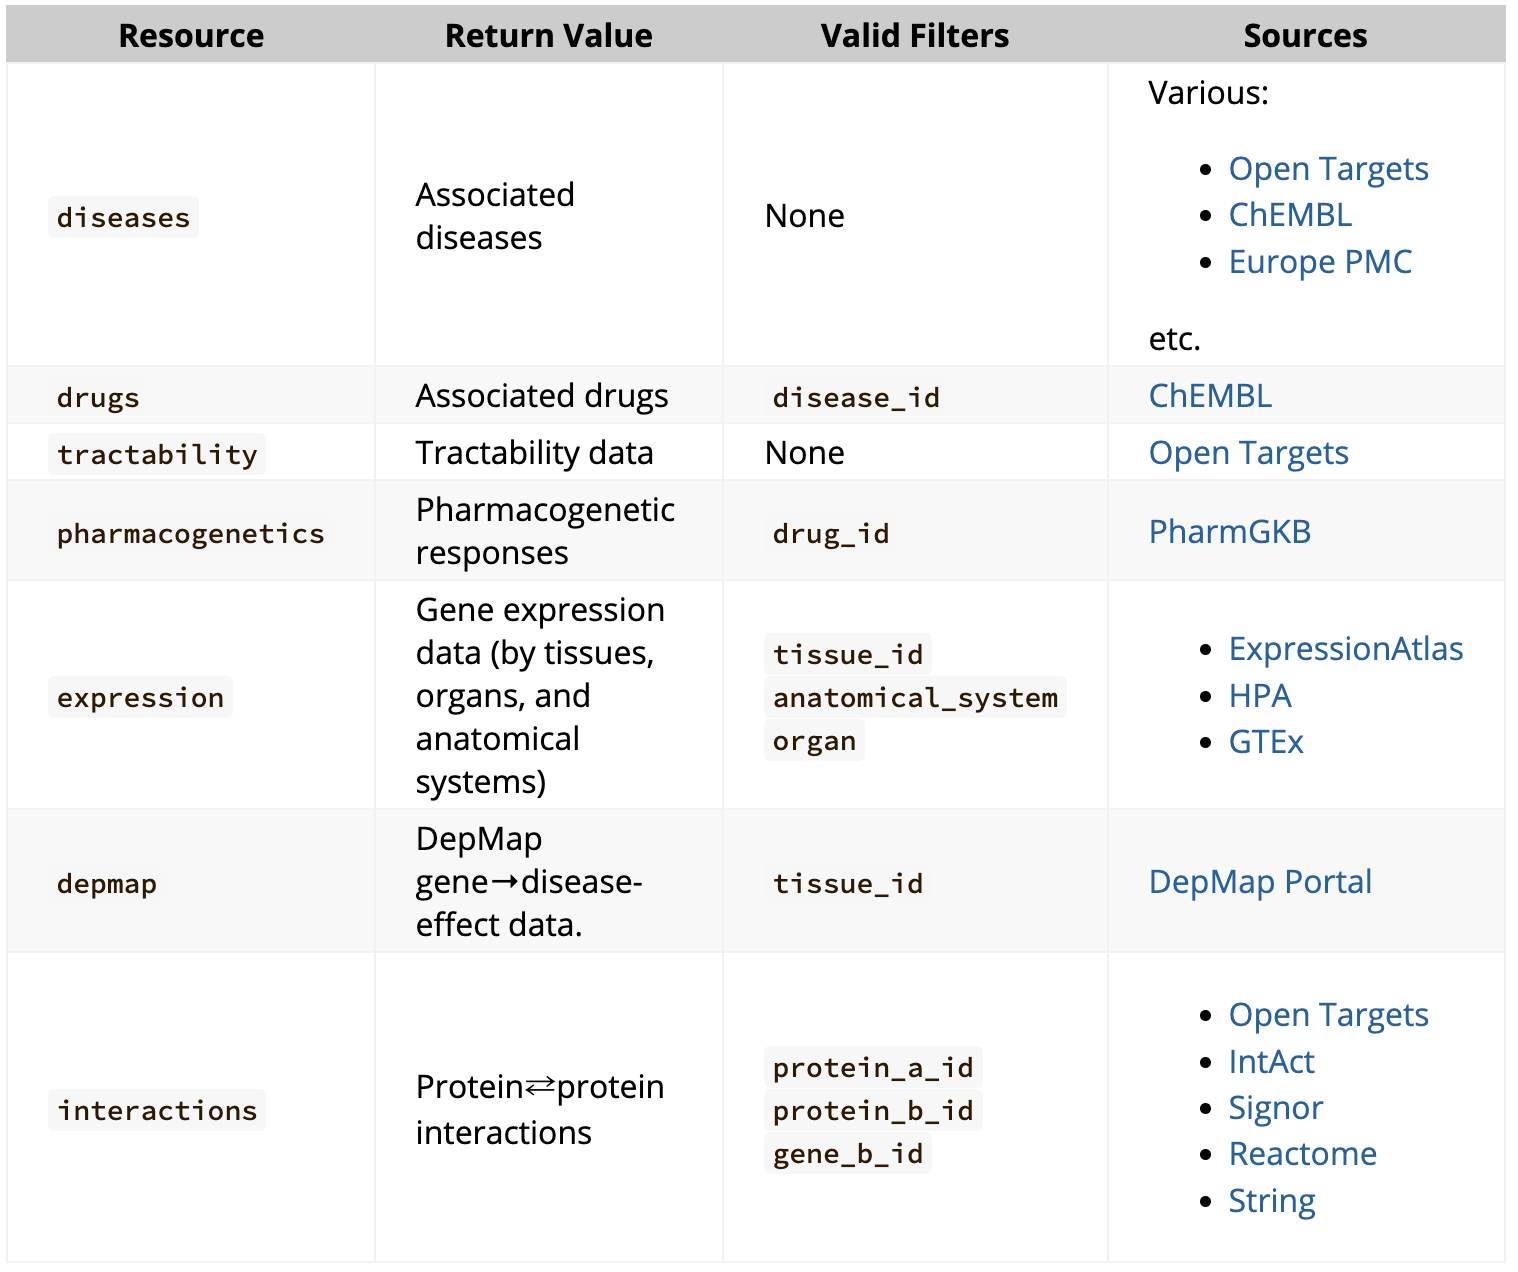
\includegraphics[width=\textwidth]{gget-opentargets-resources.png}
      \end{figure}
    \end{column}
    \begin{column}{0.6\textwidth}
      \begin{itemize}
      \item \texttt{\textbf{opentargets}} fetches resources using
        Ensembl IDs
      \item \texttt{\textbf{sc.queries.biomart\_annotations()}}
        identified 152 Ensemble IDs for 115 human lung cell atlas
        NSForest marker gene symbols
      \item Fetched diseases, drugs, interactions, tractability,
        expression, and depmap resources
      \item Obtained 6,520 diseases, and 102 drugs, so filtered drugs
        by score $\ge$ 0.5 to limit to 175 diseases
      \end{itemize}
    \end{column}
  \end{columns}
\end{frame}

\begin{frame}
  \frametitle{Example \textbf{disease} resource for ENSG00000239961}
  \framesubtitle{NSForest marker LILRA4 for Plasmacytoid DCs}
  \begin{enumerate}\footnotesize
  \item[]\textbf{id:} EFO\_0007937
  \item[]\textbf{name:} blood protein measurement
  \item[]\textbf{description:} quantification of the levels of some
    protein in a blood sample
  \item[]\textbf{score:} 0.3370941177
  \end{enumerate}
\end{frame}

\begin{frame}
  \frametitle{Example \textbf{drug} resource for ENSG00000239961}
  \framesubtitle{NSForest marker LILRA4 for Plasmacytoid DCs}
  \begin{columns}[t]\footnotesize
    \begin{column}{0.5\textwidth}
      \begin{enumerate}
      \item[]\textbf{id:} CHEMBL4594330
      \item[]\textbf{name:} DAXDILIMAB
      \item[]\textbf{type:} Antibody
      \item[] \textbf{action mechanism} Leukocyte immunoglobulin-like
        receptor subfamily A member 4 inhibitor
      \item[]\textbf{description:} Antibody drug with a maximum clinical
        trial phase of II (across all indications) and has 7
        investigational indications
      \end{enumerate}
    \end{column}
    \begin{column}{0.5\textwidth}
      \begin{enumerate}
      \item[]\textbf{synonyms:} Daxdilimab, HZN-7734, MEDI-7734, MEDI7734,
        Medi 7734, Medi7734, VIB7734, Vib-7734, Vib7734
      \item[]\textbf{trade names:} none
      \item[]\textbf{disease id:} MONDO\_0019558
      \item[]\textbf{disease name:} discoid lupus erythematosus
      \item[]\textbf{trialphase} 2
      \item[]\textbf{trial status} Recruiting
      \item[]\textbf{trial ids} NCT0559122
      \item[]\textbf{approved:} false
      \end{enumerate}
    \end{column}
  \end{columns}
\end{frame}

\begin{frame}
  \frametitle{Example \textbf{protein-protein interaction} resource for ENSG00000239961}
  \framesubtitle{NSForest marker LILRA4 for Plasmacytoid DCs}
  \begin{columns}[t]\footnotesize
    \begin{column}{0.5\textwidth}
      \begin{enumerate}
      \item[]\textbf{protein a id:} ENSP00000291759
      \item[]\textbf{gene a id:} ENSG00000239961
      \item[]\textbf{gene a symbol:} LILRA4
      \item[]\textbf{role a:} unspecified role
      \item[]\textbf{taxon a:} 9606
      \item[]\textbf{evidence score:} 0.995
      \item[]\textbf{evidence count:} 3
      \item[]\textbf{source db:} string
      \end{enumerate}
    \end{column}
    \begin{column}{0.5\textwidth}
      \begin{enumerate}
      \item[]\textbf{protein b id:} ENSP00000252593
      \item[]\textbf{gene b id:} ENSG00000130303
      \item[]\textbf{gene b symbol:} BST2
      \item[]\textbf{role b:} unspecified role
      \item[]\textbf{taxon b:} 9606
      \end{enumerate}
    \end{column}
  \end{columns}
\end{frame}

\begin{frame}
  \frametitle{Example \textbf{tractability} resources for ENSG00000239961}
  \framesubtitle{NSForest marker LILRA4 for Plasmacytoid DCs}
  \begin{enumerate}\footnotesize
  \item[]\textbf{label:} Advanced Clinical, \textbf{modality:} Antibody
  \item[]\textbf{label:} UniProt loc high conf, \textbf{modality:} Antibody
  \item[]\textbf{label:} GO CC high conf, \textbf{modality:} Antibody
  \item[]\textbf{label:} UniProt SigP or TMHMM, \textbf{modality:} Antibody
  \item[]\textbf{label:} Half-life Data, \textbf{modality:} PROTAC
  \end{enumerate}
\end{frame}

\begin{frame}
  \frametitle{Example \textbf{gene expression} resource for ENSG00000239961}
  \framesubtitle{NSForest marker LILRA4 for Plasmacytoid DCs}
  \begin{enumerate}\footnotesize
  \item[]\textbf{tissue id:} CL 0000738
  \item[]\textbf{tissue name:} leukocyte
  \item[]\textbf{rna zscore:} 4
  \item[]\textbf{rna value:} 921.0
  \item[]\textbf{rna unit:} 
  \item[]\textbf{rna level:} 3
  \item[]\textbf{anatomical systems:} hematopoietic system, immune system
  \item[]\textbf{organs:} immune organ
  \end{enumerate}
\end{frame}

\begin{frame}
  \frametitle{Example \textbf{gene-disease effect (depmap)} resource for ENSG00000239961}
  \framesubtitle{NSForest marker LILRA4 for Plasmacytoid DCs}
  \begin{enumerate}\footnotesize
  \item[]\textbf{depmap id:} ACH-001303
  \item[]\textbf{expression:} 0.0
  \item[]\textbf{effect:} 0.08098055
  \item[]\textbf{tissue id:} UBERON 0000010
  \item[]\textbf{tissue name:} Peripheral Nervous System
  \item[]\textbf{cell line name:} NB-1643
  \item[]\textbf{disease cell line id:} null
  \item[]\textbf{disease name:} Neuroblastoma
  \item[]\textbf{mutation:} null
  \end{enumerate}
\end{frame}

\begin{frame}
  \frametitle{Publication - Cell-set - Gene - Biomarker-combination network}
  \framesubtitle{}
  \begin{itemize}\tiny
  \item[] (biomarker combination, IS\_MARKER\_FOR, cell set): One
    biomarker combination vertex for both publications, if identical
  \item[] (cell type, PART\_OF, anatomic structure)
  \item[] (cell set, IS\_INSTANCE, cell type): Distinct cell set
    vertices for each publication, even if identical
  \item[] (cell set, EXPRESSES, gene\_name)
  \item[] (cell set, SOURCE, publication)
  \item[] (gene\_name, PART\_OF, biomarker combination)
  \end{itemize}
  \begin{figure}
    \begin{center}
      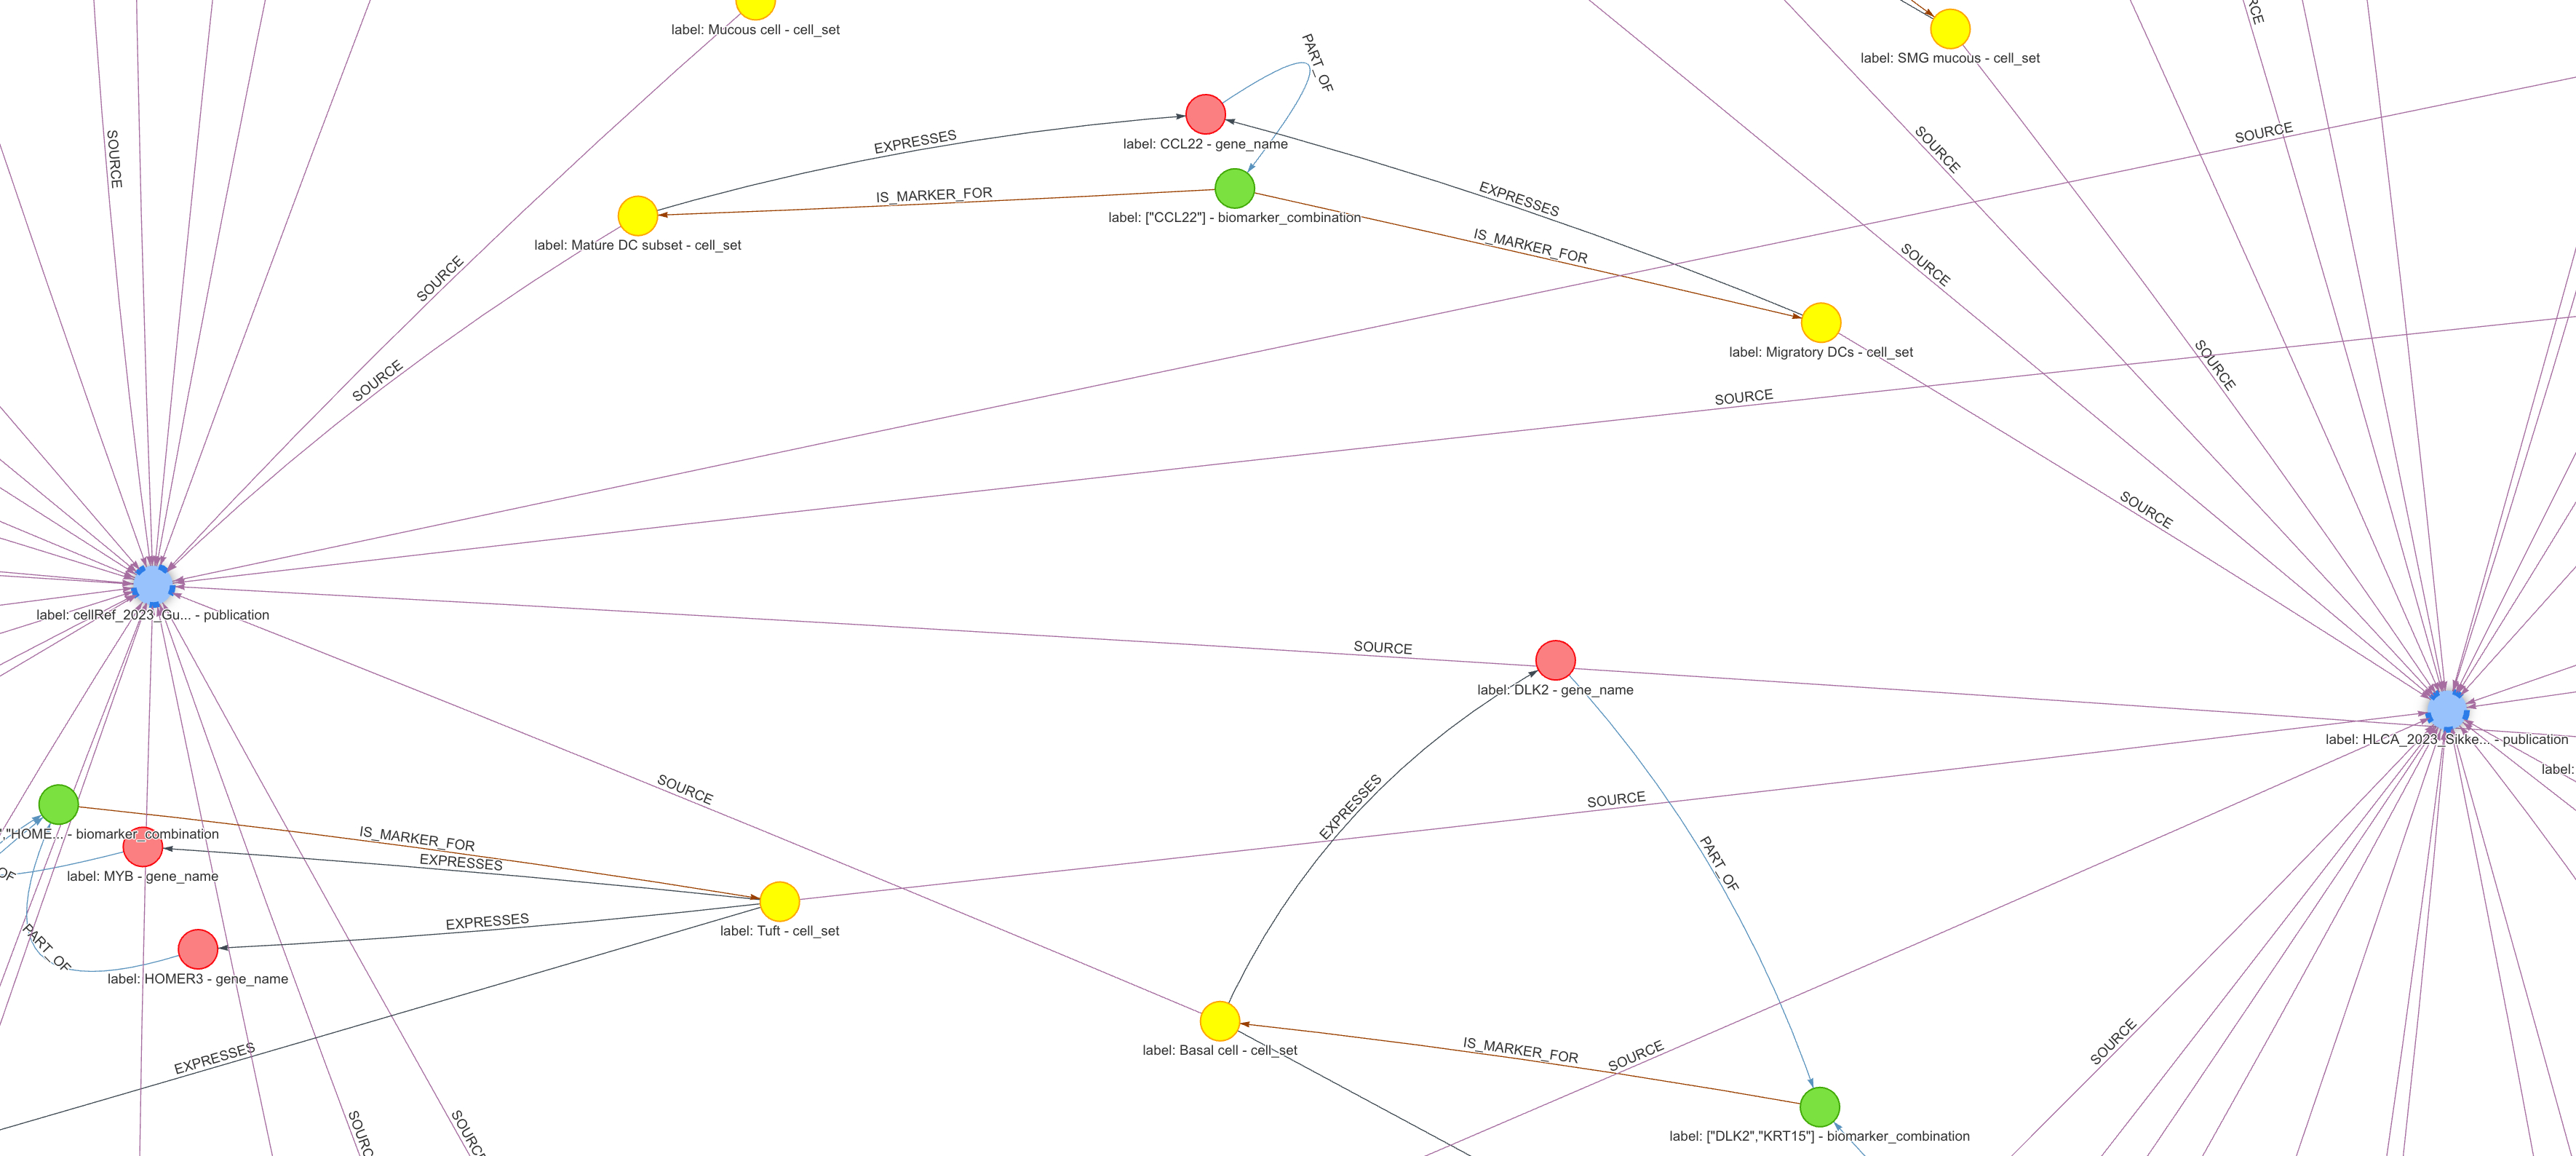
\includegraphics[height=0.6\textheight]{publication-cell-set-gene-biomarker-combination.jpeg}
    \end{center}
  \end{figure}
\end{frame}

\begin{frame}
  \frametitle{Gene - Drug - Disease network}
  \framesubtitle{}
  \begin{itemize}\tiny
  \item[] (gene name, IS\_BASIS\_FOR\_CONDITION, disease)
  \item[] (drug product, MOLECULARLY\_INTERACTS\_WITH, gene name)
  \item[] (drug product, IS\_SUBSTANCE\_THAT\_TREATS, disease)
  \end{itemize}
  \begin{figure}
    \begin{center}
      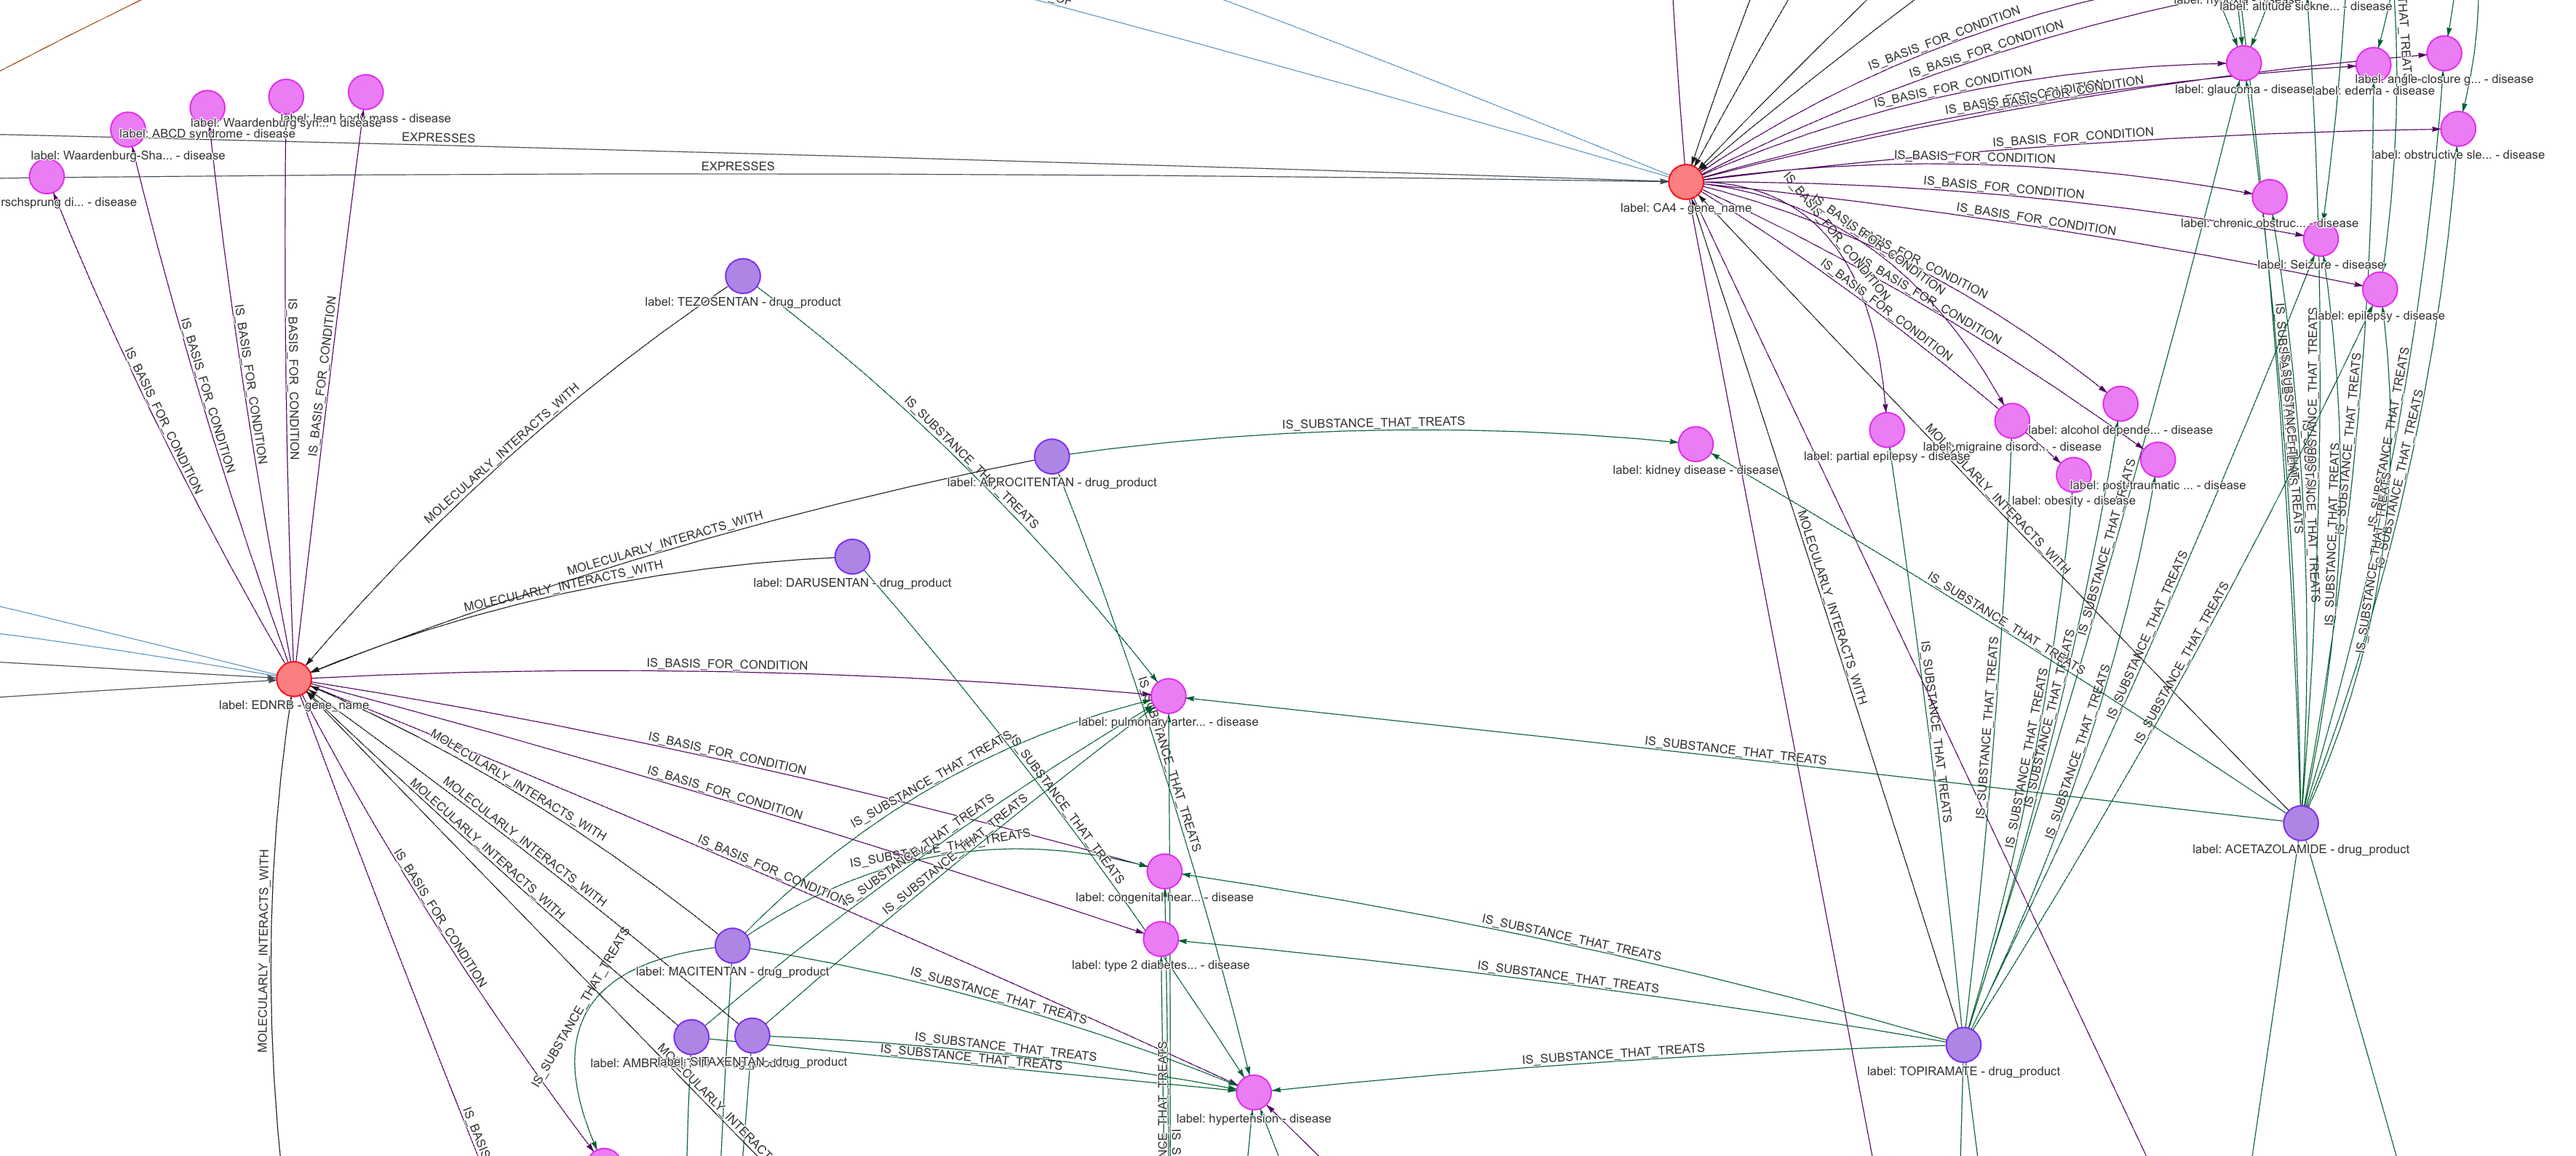
\includegraphics[height=0.6\textheight]{gene-drug-disease.jpeg}
    \end{center}
  \end{figure}
\end{frame}

%% cell\_set-publication
%% cell\_set-CL

%% cell\_set-publication
%% biomarker\_combination-cell\_set
%% gene\_name-biomarker\_combination

%% cell\_set-publication
%% biomarker\_combination-cell\_set
%% gene\_name-biomarker\_combination
%% gene\_name-disease from one shared gene and filter out EFO

%% cell\_set-publication
%% biomarker\_combination-cell\_set
%% gene\_name-biomarker\_combination
%% drug\_product-gene\_name from one shared gene

%% f
%% \begin{frame}
%%   \frametitle{}
%%   \framesubtitle{}
%% \end{frame}

%% i
%% \begin{itemize}
%% \item[]
%% \end{itemize}

%% e
%% \begin{enumerate}
%% \item
%% \item
%% \end{enumerate}

%% c
%% \begin{columns}
%%   \begin{column}{0.5\textwidth}
%%   \end{column}
%%   \begin{column}{0.5\textwidth}
%%   \end{column}
%% \end{columns}

%% g
%% \begin{frame}
%%   \frametitle{}
%%   \framesubtitle{}
%%   \begin{figure}
%%     \begin{center}
%%       \includegraphics[height=0.8\textheight]{}
%%     \end{center}
%%   \end{figure}
%% \end{frame}

%% b
%% \begin{frame}
%%   \frametitle{}
%%   \framesubtitle{}
%%   \begin{table}
%%     \begin{center}
%%       \input{}
%%     \end{center}
%%   \end{table}
%% \end{frame}

\end{document}
